\documentclass[9pt]{beamer}
\usepackage{amsmath}
\usepackage{amssymb}
\usepackage{graphicx}
\usepackage{tikz}
\usetikzlibrary{shapes.geometric, arrows}
\usetikzlibrary{positioning}
\definecolor{orange}{RGB}{235,113,37}

\tikzstyle{IO} = [rectangle, rounded corners, minimum width=2cm, minimum height=1 cm , text centered, draw=black, fill=red!30]
\tikzstyle{process} = [rectangle, minimum width=2cm, minimum height=1 cm , text centered, draw=black, fill=orange]
\tikzstyle{arrow} = [thick, ->, >=stealth]


\usetheme{default}
\usecolortheme{default}

\title{Synthesized PTZ}
\author{Adrian and Filip}

\begin{document}
\maketitle
\begin{frame}
	\frametitle{table of Contents}
	\tableofcontents
\end{frame}

\section{implementation}
\begin{frame}
	\frametitle{implementation}
	\begin{tikzpicture}[node distance=1.2cm]
		\node (input4) [IO] {User input};
		\node (input1) [IO, right of= input4, xshift=1.7cm] {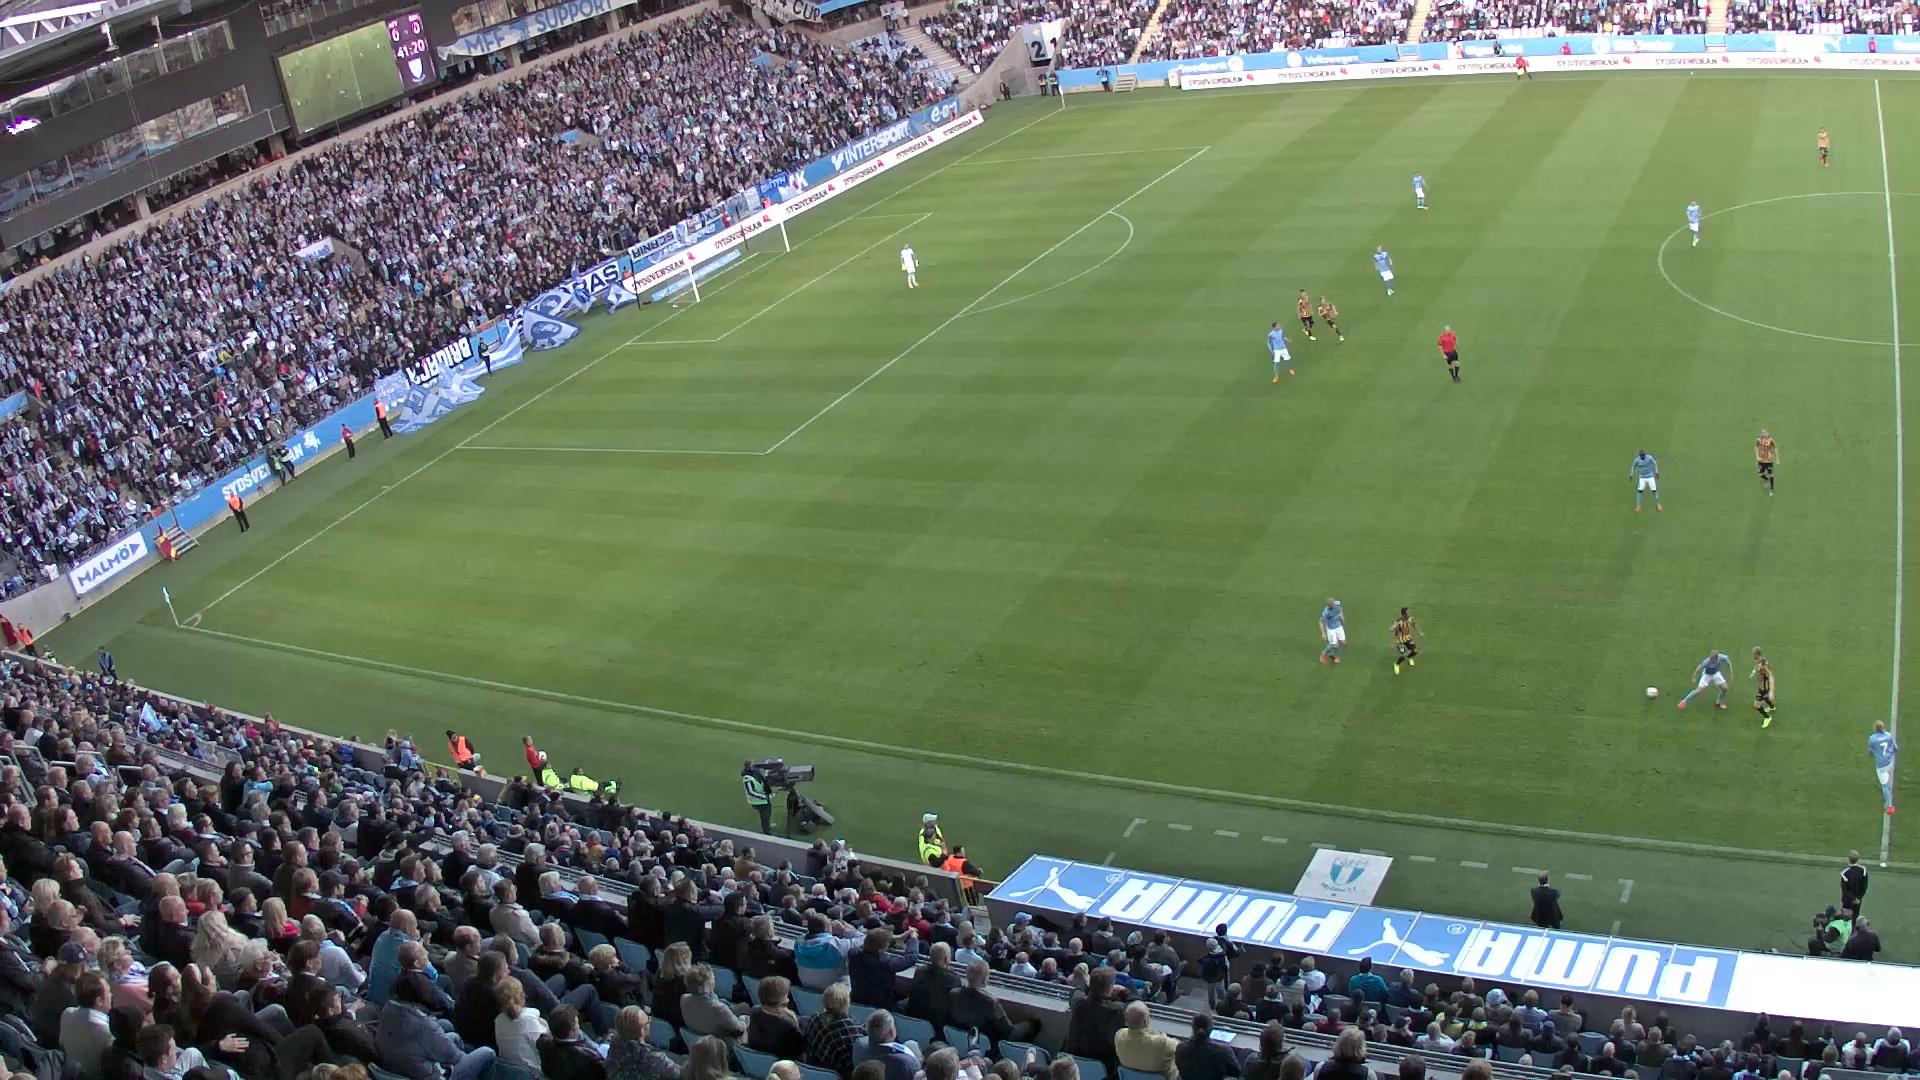
\includegraphics[width=2cm]{../data/20150521_194353_C1D8.jpg}};
		\node (input2) [IO, right of= input1, xshift=1.3cm] {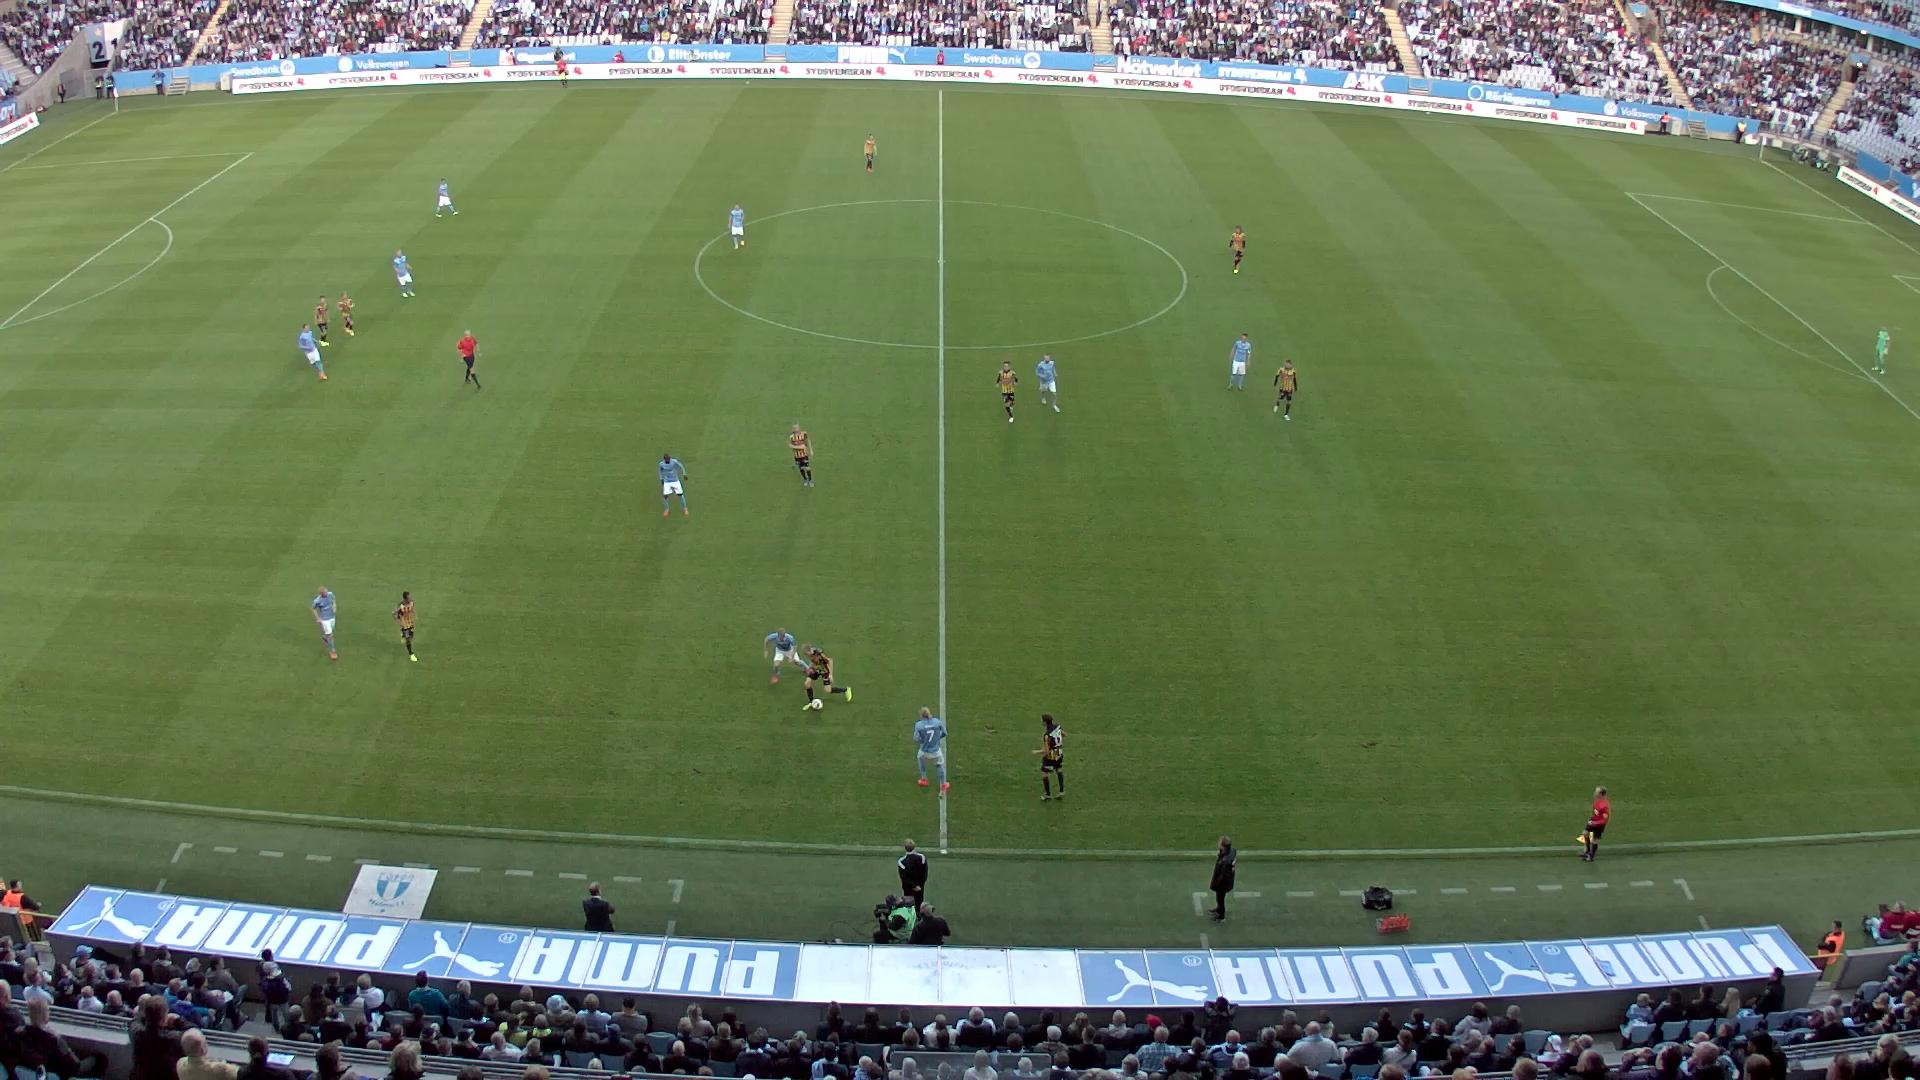
\includegraphics[width=2cm]{../data/20150521_194353_FD1E.jpg}};
		\node (input3) [IO, right of= input2, xshift=1.3cm] {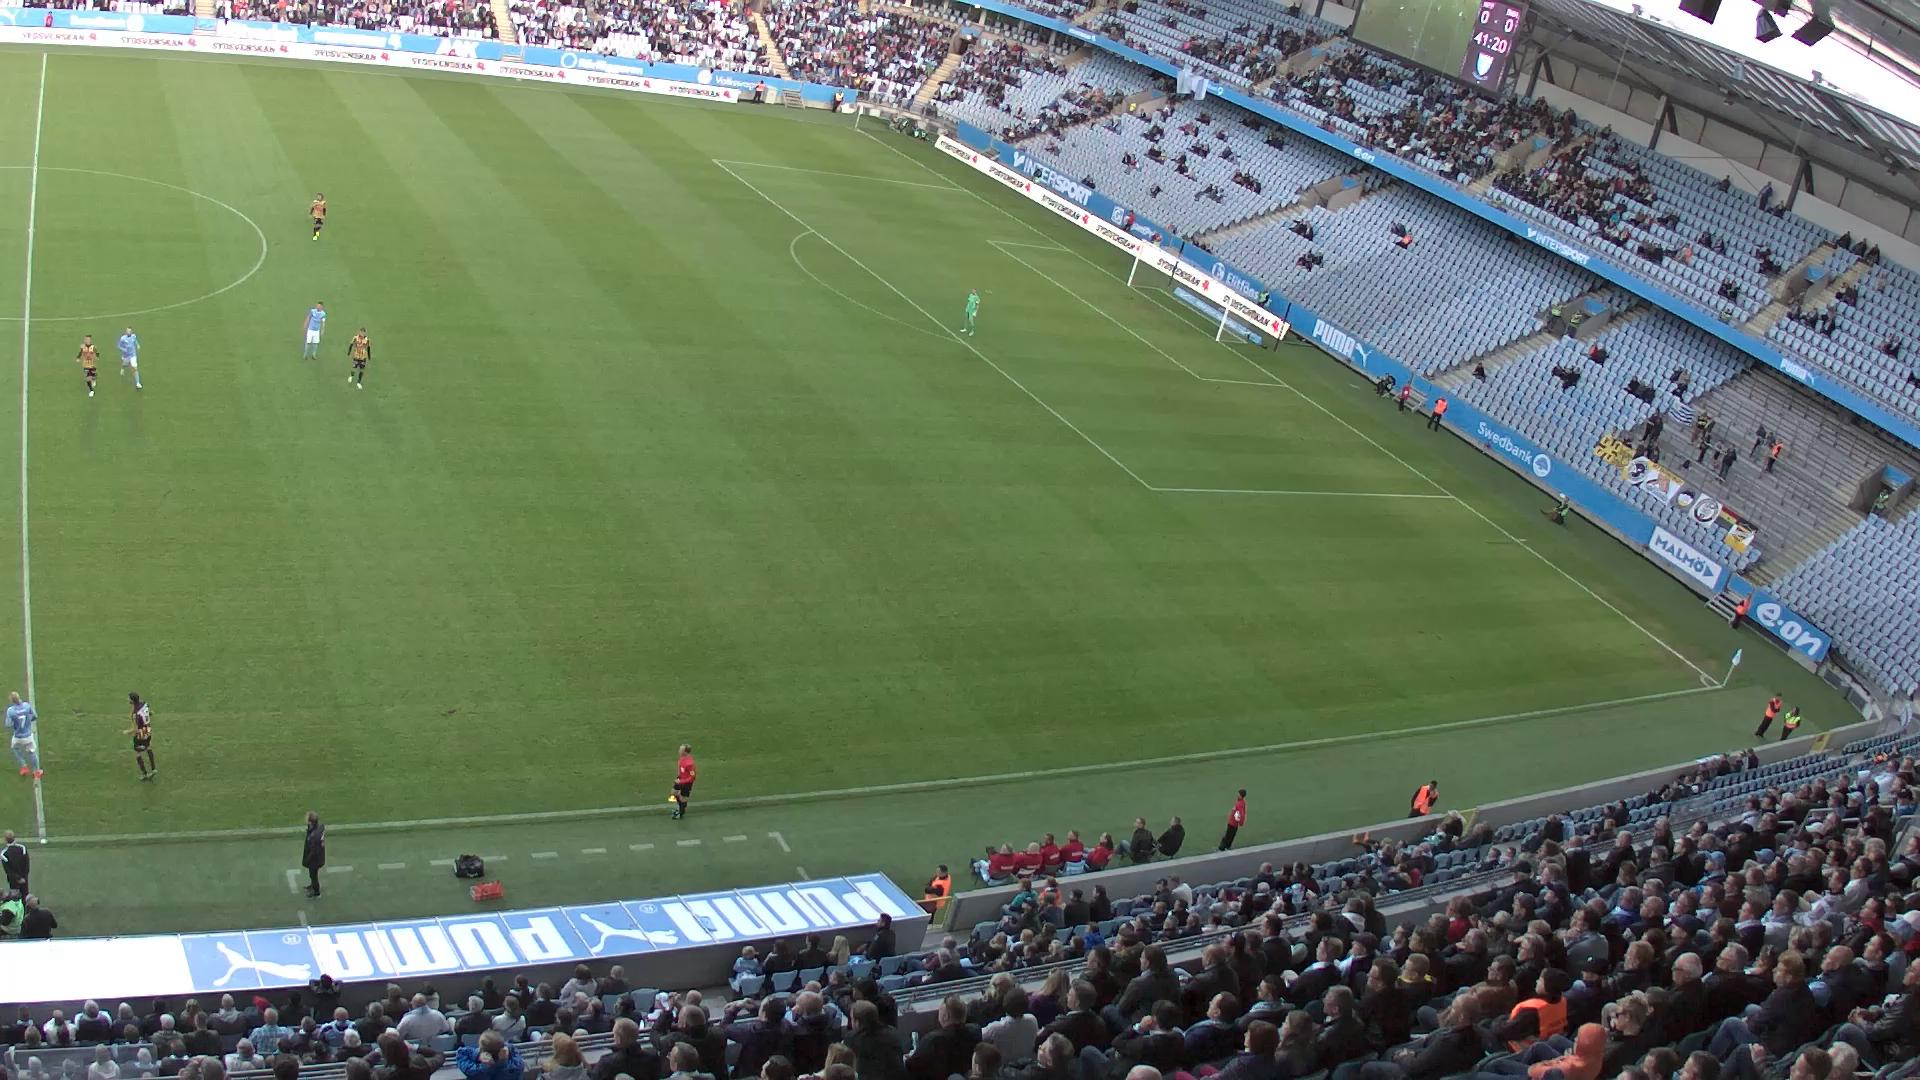
\includegraphics[width=2cm]{../data/20150521_194353_49E3.jpg}};
		\node (SURF1) [process, below of= input1, yshift=-0.2cm] {Extract SURF features};
		\node (SURF2) [process, below of= input3, yshift=-0.2cm] {Extract SURF features};
		\node (Homo1) [process, below of= SURF1] {Homography to center image};
		\node (Homo2) [process, below of= SURF2] {Homography to center image};
		\node (PTZ) [process, below of= input4, yshift=-0.2cm] {PTZ matrix};
		\node (Trans) [process, below of= PTZ,yshift=-1.3cm] {Apply transformations};
		\node (Blend) [process, below of=Trans, yshift=-0.5cm] {Blend results};
		\node (Output) [IO, right of=Blend, xshift=4.5cm] {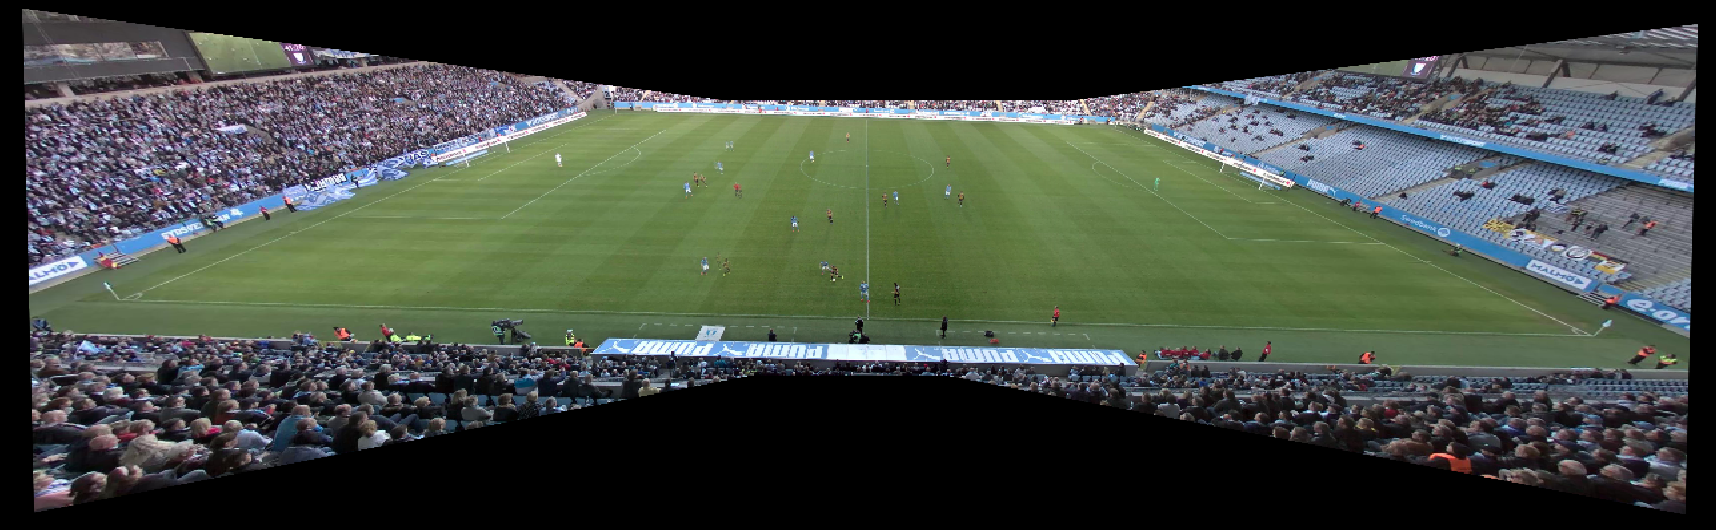
\includegraphics[width=7cm]{../results/images/res_stitch.PNG}};
		\draw [arrow] (input1) -- (SURF1);
		\draw [arrow] (input3) -- (SURF2);
		\draw [arrow] (input4) -- (PTZ);
		\draw [arrow] (SURF1) -- (Homo1);
		\draw [arrow] (SURF2) -- (Homo2);
		\draw [arrow] (PTZ)  -- (Trans);
		\draw [arrow] (Homo1)  |- (Trans);
		\draw [arrow] (Homo2)  |- (Trans);
		\draw [arrow] (input2) |- (Trans);
		\draw [arrow] (Trans) -- (Blend);
		\draw [arrow] (Blend) -- (Output);
	\end{tikzpicture}

\end{frame}

\end{document}

